% Project Report : Group 02

\documentclass[english, 11pt]{article}
\usepackage{times}
\usepackage[top=1.0in, bottom=1.0in, left=0.5in, right=0.5in]{geometry}
\usepackage{graphicx}
\usepackage{babel}
%\usepackage{siunitx}

\begin{document}

\title{CS296 Project Report : Group 02}

% Author's Name Goes Here
\author{Shubham Jain\\ % Newline
	120050002\\
	shubhamj@cse.iitb.ac.in\\
	\\	
	Palash Kala\\
	120050010\\
	palashk@cse.iitb.ac.in\\
	\\
	Tapish Raniwal\\
	120050023\\
	tapish@cse.iitb.ac.in\\}

% Today will be replaced with current date
\date{\today}

\maketitle % Without this tag the above information will not appear in the generated document

\section{Introduction}

This report has been made to provide the original design and the final design of our project "Shrimp Rover : All Terrain Bot" 
and to discuss the differences between them. This report also includes an analysis of the submitted code as well as a 
discussion about its performance.

\section{Design}

\subsection{Final Design}
\begin{figure}
	\begin{center}
		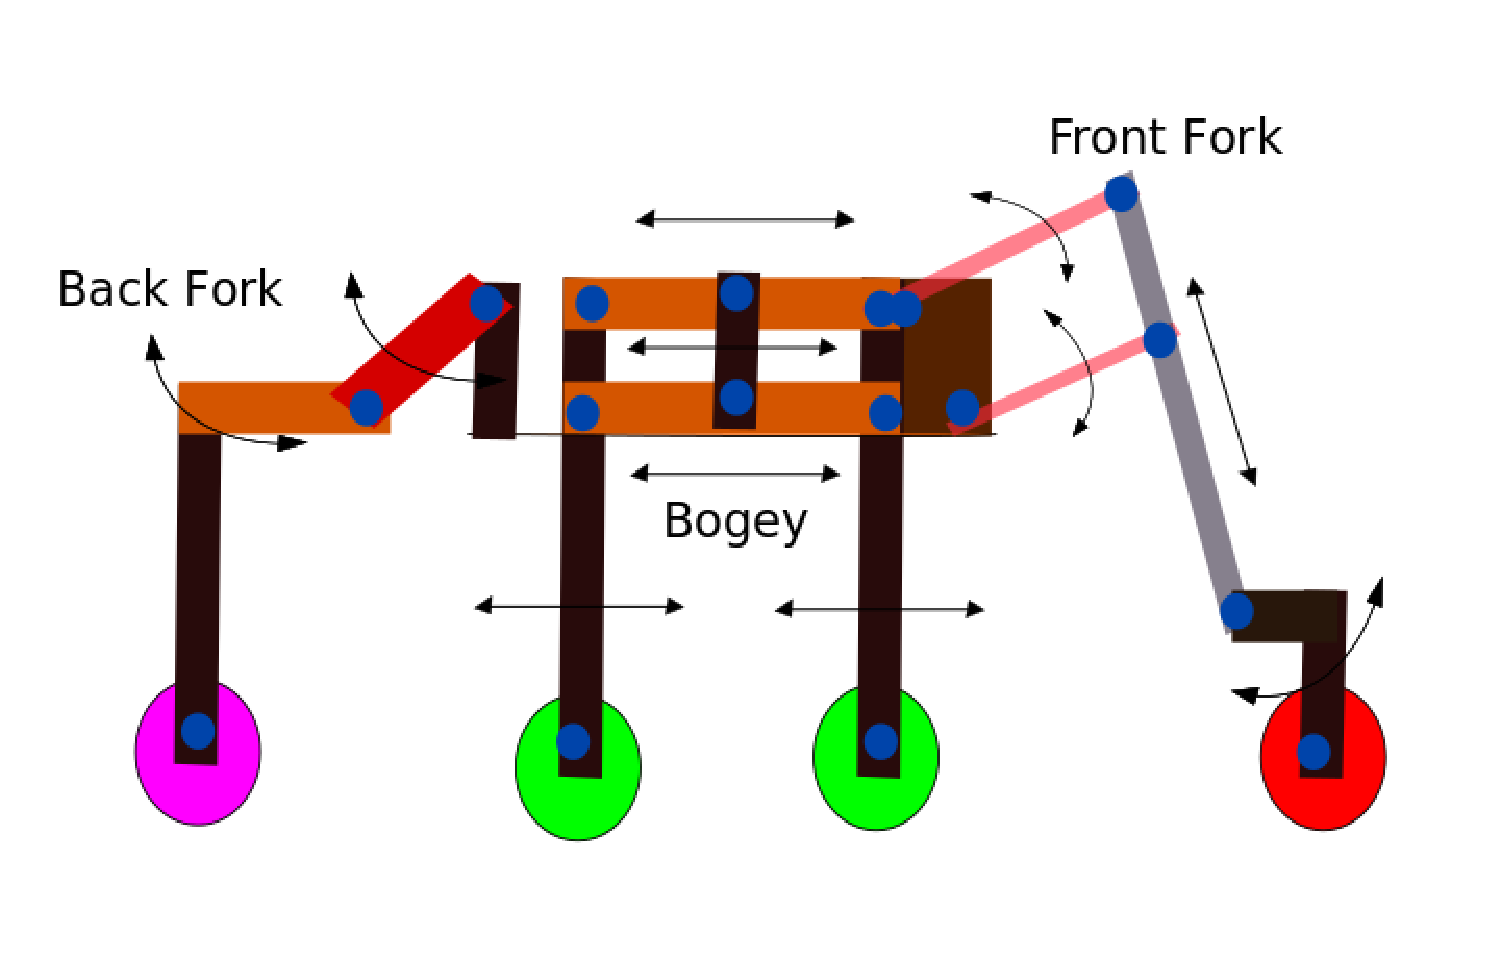
\includegraphics[width=400px]{drawing}
	\end{center}
	\caption{Shrimp Rover : Original Design}
\end{figure}

The original design of our project depicts a shrimp rover bot. This
bot is an all terrain bot which can go through hills, mountains, roads, slope, etc.
This bot had around 17 simple moving parts of which some parts are able to rotate back and forth.
It consisted of a central bogey , front fork, back fork and wheels. 

\subsection{Final Design}
\begin{figure}
	\begin{center}
		\includegraphics[width=400px]{screenshot1}
	\end{center}
	\caption{Shrimp Rover : Final Design}
\end{figure}

The final design is almost similar to the original design. The final design has some more components 
as compared to the original design, as we put a spring between the two rods attching the central bogey to the front fork.
 The final design is made after many trials of different measurements of friction, density and sizes of rods. \\
 Its Spring suspension guarantees optimal ground contact of all wheels at any time and its parallel mechanism produces a passive elevation 
 of the front wheel if an obstacle is encountered.\\
 The bogies provide the lateral stability. \\
\subsection{Final Design}
\begin{figure}
	\begin{center}
		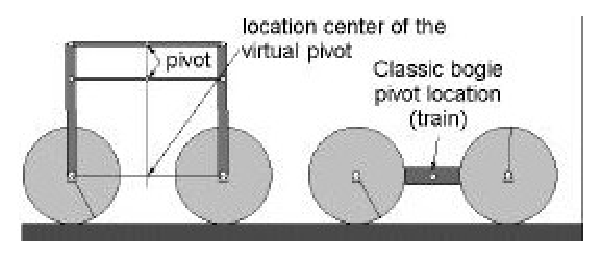
\includegraphics[width=400px]{mechanism1}
	\end{center}
	\caption{Shrimp Rover : Bogie}
\end{figure}
 
 The body of the bot is made such that centre of mass is shifted towards the front wheel which
increases the climbing capacity of the bot.

\subsection{Final Design}
\begin{figure}
	\begin{center}
		\includegraphics[width=400px]{screenshot1}
	\end{center}
	\caption{Shrimp Rover : Final Design}
\end{figure}

 

\subsection{Interesting Things}
The design consists of a lot of interesting things. Even after such a simple structure, it is able to cross many terrains because of its structure and measurements. 
The parallel architecture of the bogies and the spring suspended fork provide a high ground clearance while
keeping all 4 wheels (actually 6 wheels in physical bot) in ground-contact at any time. This ensures excellent climbing capabilities over
obstacles much higher than the wheel radius and an excellent adaptation to all sorts of terrains.\cite{ieeepaper} \\
The body of the bot is made such that the center of mass is shifted towards the front wheel which increases the climbing capacity of the bot.\\
The first tyre uses the energy stored in the spring to rise up and then the second tyre rises up. After this, as the center of mass is higher\\
 the third and fourth tyres go up easily.\cite{book1} \\
 \begin{figure}
	\begin{center}
		\includegraphics[width=400px]{high}
	\end{center}
	\caption{The energy is stored in the spring}
\end{figure}
 
\section{Analysis Of Code}

\subsection{Profiling}

Release Prof O2:\\
Number of Iterations: 10000\\
Average time per step is 0.0351558 ms\\
Average time for collisions is 0.000746974 ms\\
Average time for position updates is 0.0117901 ms\\
Average time for velocity updates is 0.00714458 ms\\
Total loop time is 435.383 ms\\
 \begin{figure}
	\begin{center}
		\includegraphics[width=400px]{output_release_02}
	\end{center}
	\caption{Call graph for O2 release}
\end{figure}

Release Prof O3: \\
Number of Iterations: 10000\\
Average time per step is 0.0343891 ms\\
Average time for collisions is 0.000729776 ms\\
Average time for position updates is 0.0114703 ms\\
Average time for velocity updates is 0.00710644 ms\\
Total loop time is 390.961 ms\\

\begin{figure}
	\begin{center}
		\includegraphics[width=400px]{output_release_03}
	\end{center}
	\caption{Call graph for O3 release}
\end{figure}


\begin{figure}
	\begin{center}
		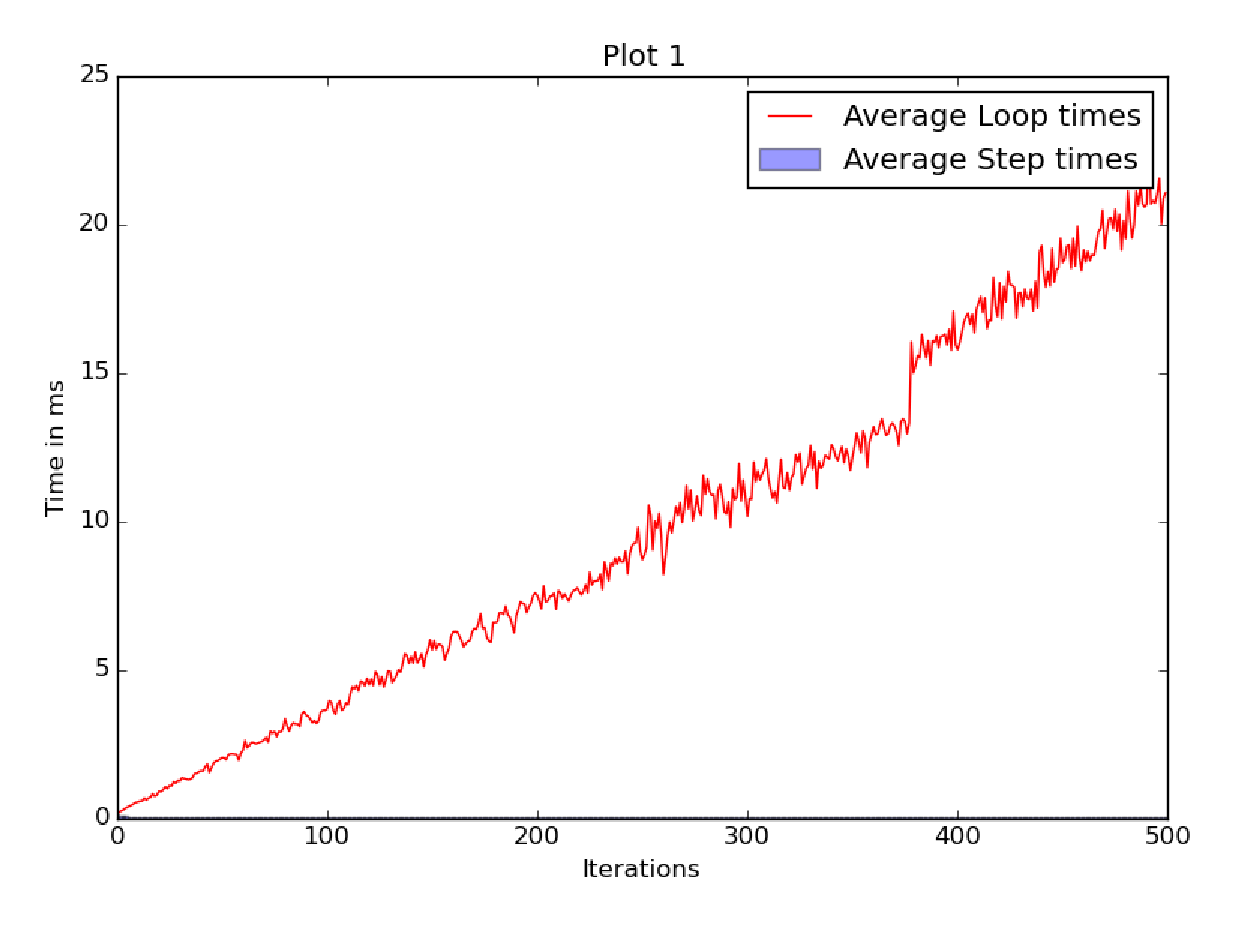
\includegraphics[width=400px]{g02_lab09_plot01}
	\end{center}
	\caption{Figure: O3 profiling}
\end{figure}

\begin{figure}
	\begin{center}
		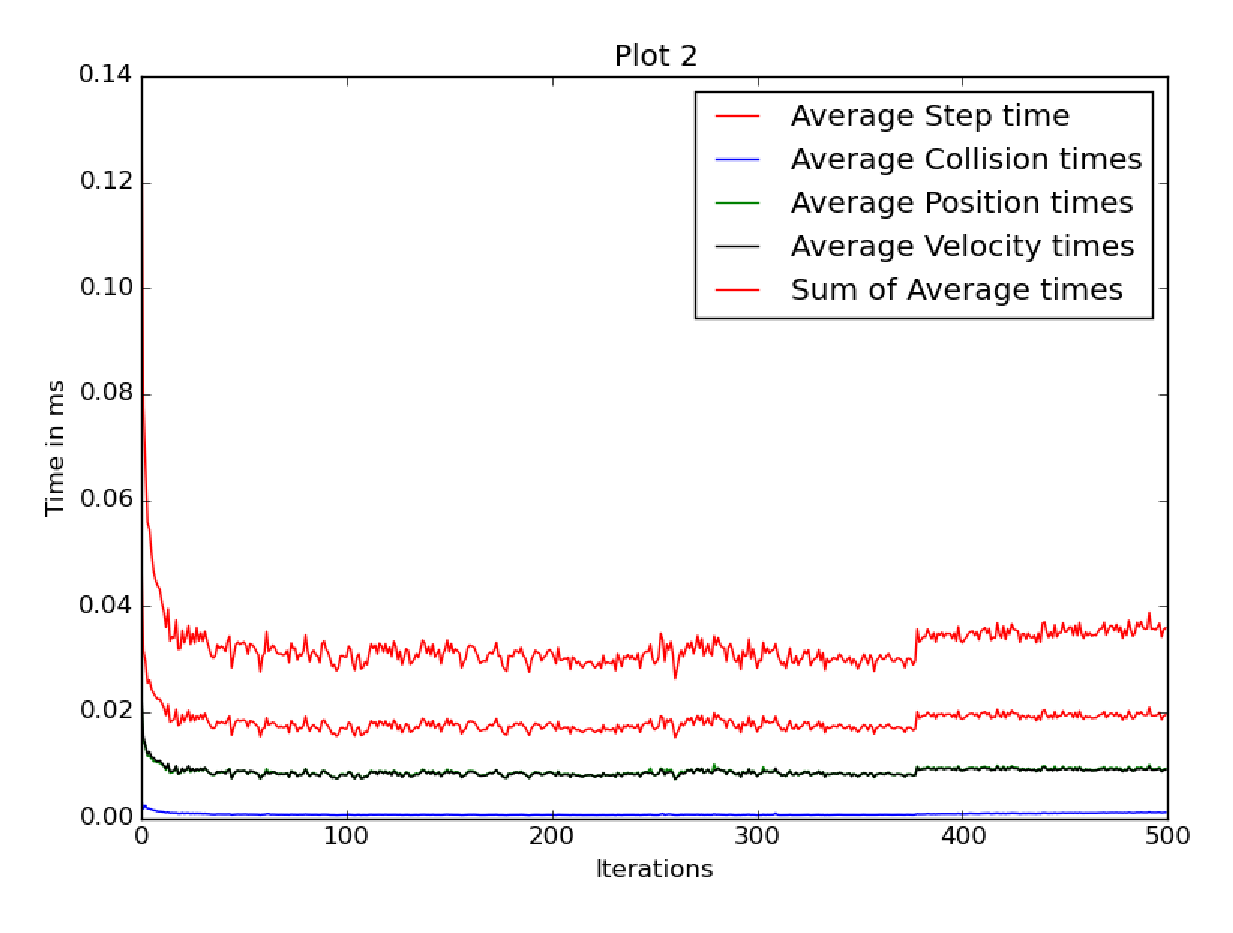
\includegraphics[width=400px]{g02_lab09_plot02}
	\end{center}
	\caption{Figure: O3 profiling}
\end{figure}

\begin{figure}
	\begin{center}
		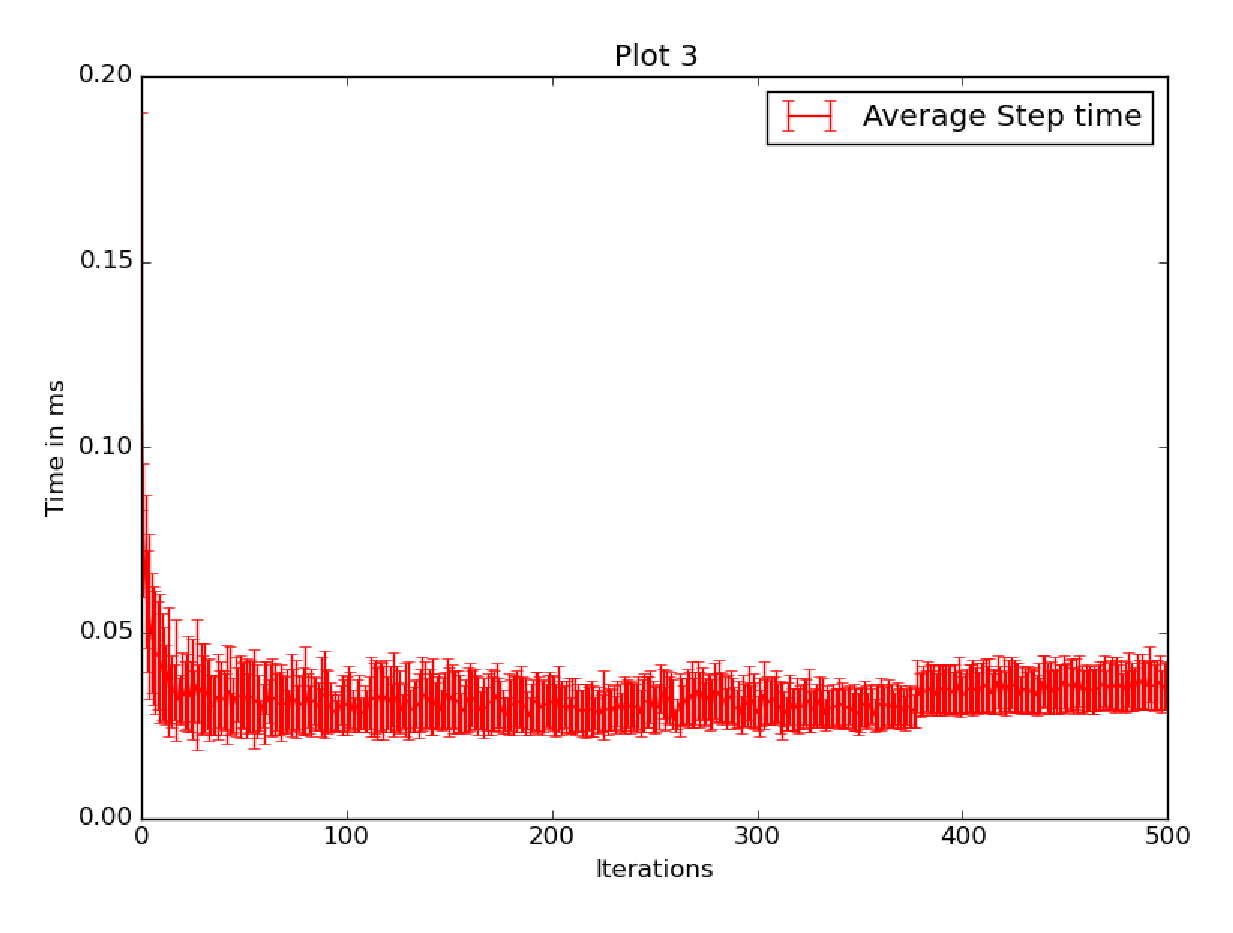
\includegraphics[width=400px]{g02_lab09_plot03}
	\end{center}
	\caption{Figure: O3 profiling}
\end{figure}

\begin{figure}
	\begin{center}
		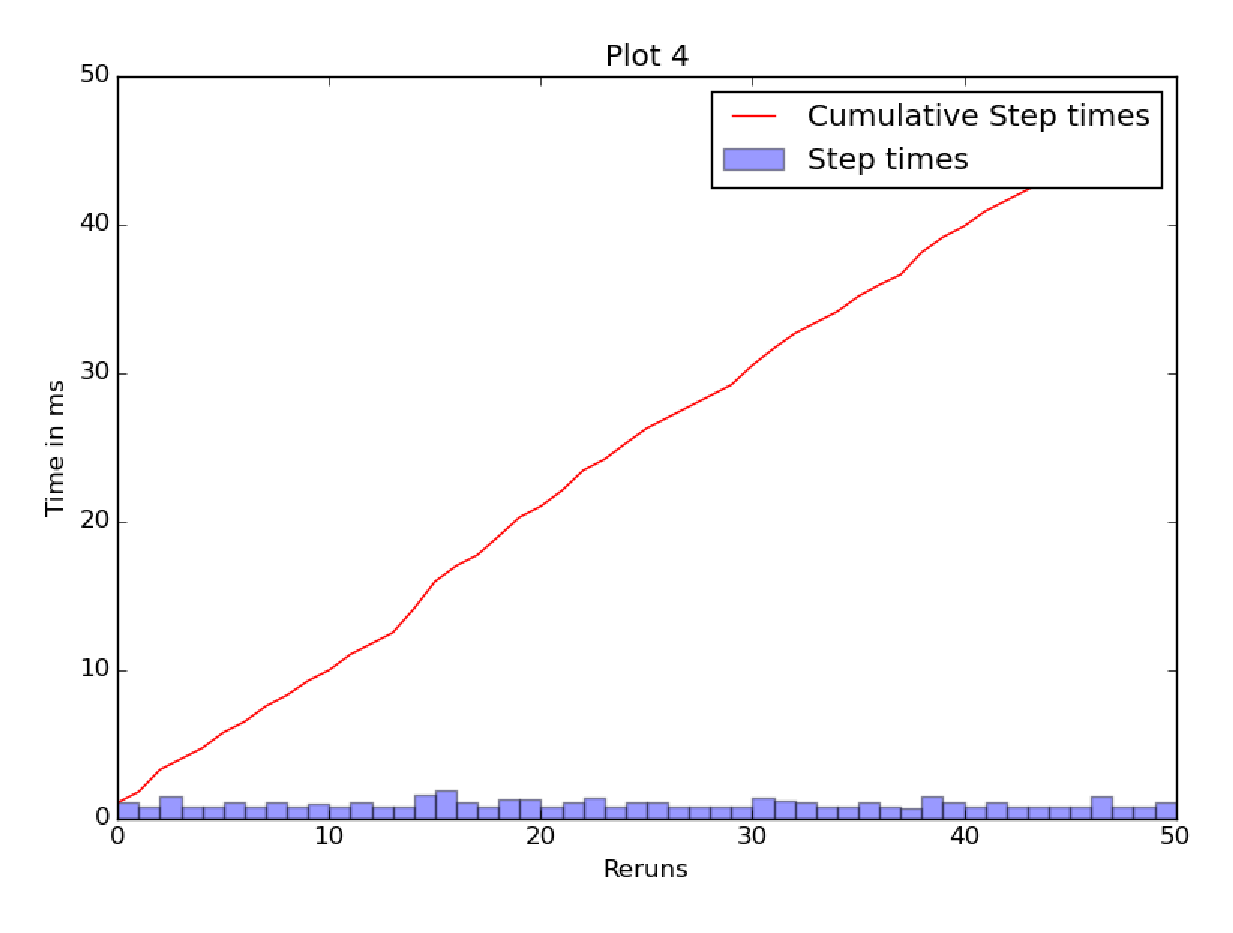
\includegraphics[width=400px]{g02_lab09_plot04}
	\end{center}
	\caption{Figure: O3 profiling}
\end{figure}

\begin{figure}
	\begin{center}
		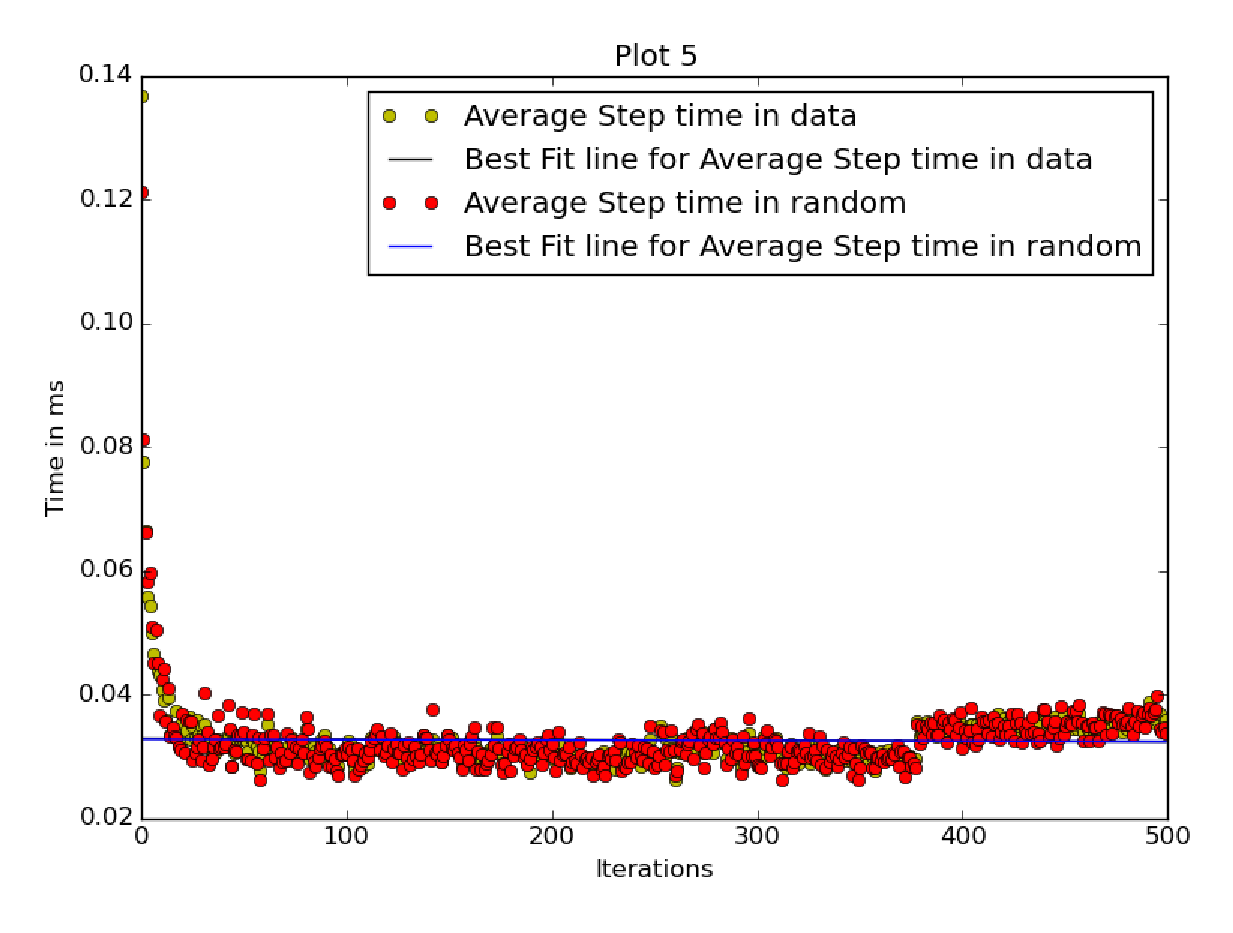
\includegraphics[width=400px]{g02_lab09_plot05}
	\end{center}
	\caption{Figure: O3 profiling}
\end{figure}

Release Prof Ofast
Number of Iterations: 10000\\
Average time per step is 0.0352842 ms\\
Average time for collisions is 0.000765978 ms\\
Average time for position updates is 0.0117918 ms\\
Average time for velocity updates is 0.00718483 ms\\
Total loop time is 401.07 ms\\

\begin{figure}
	\begin{center}
		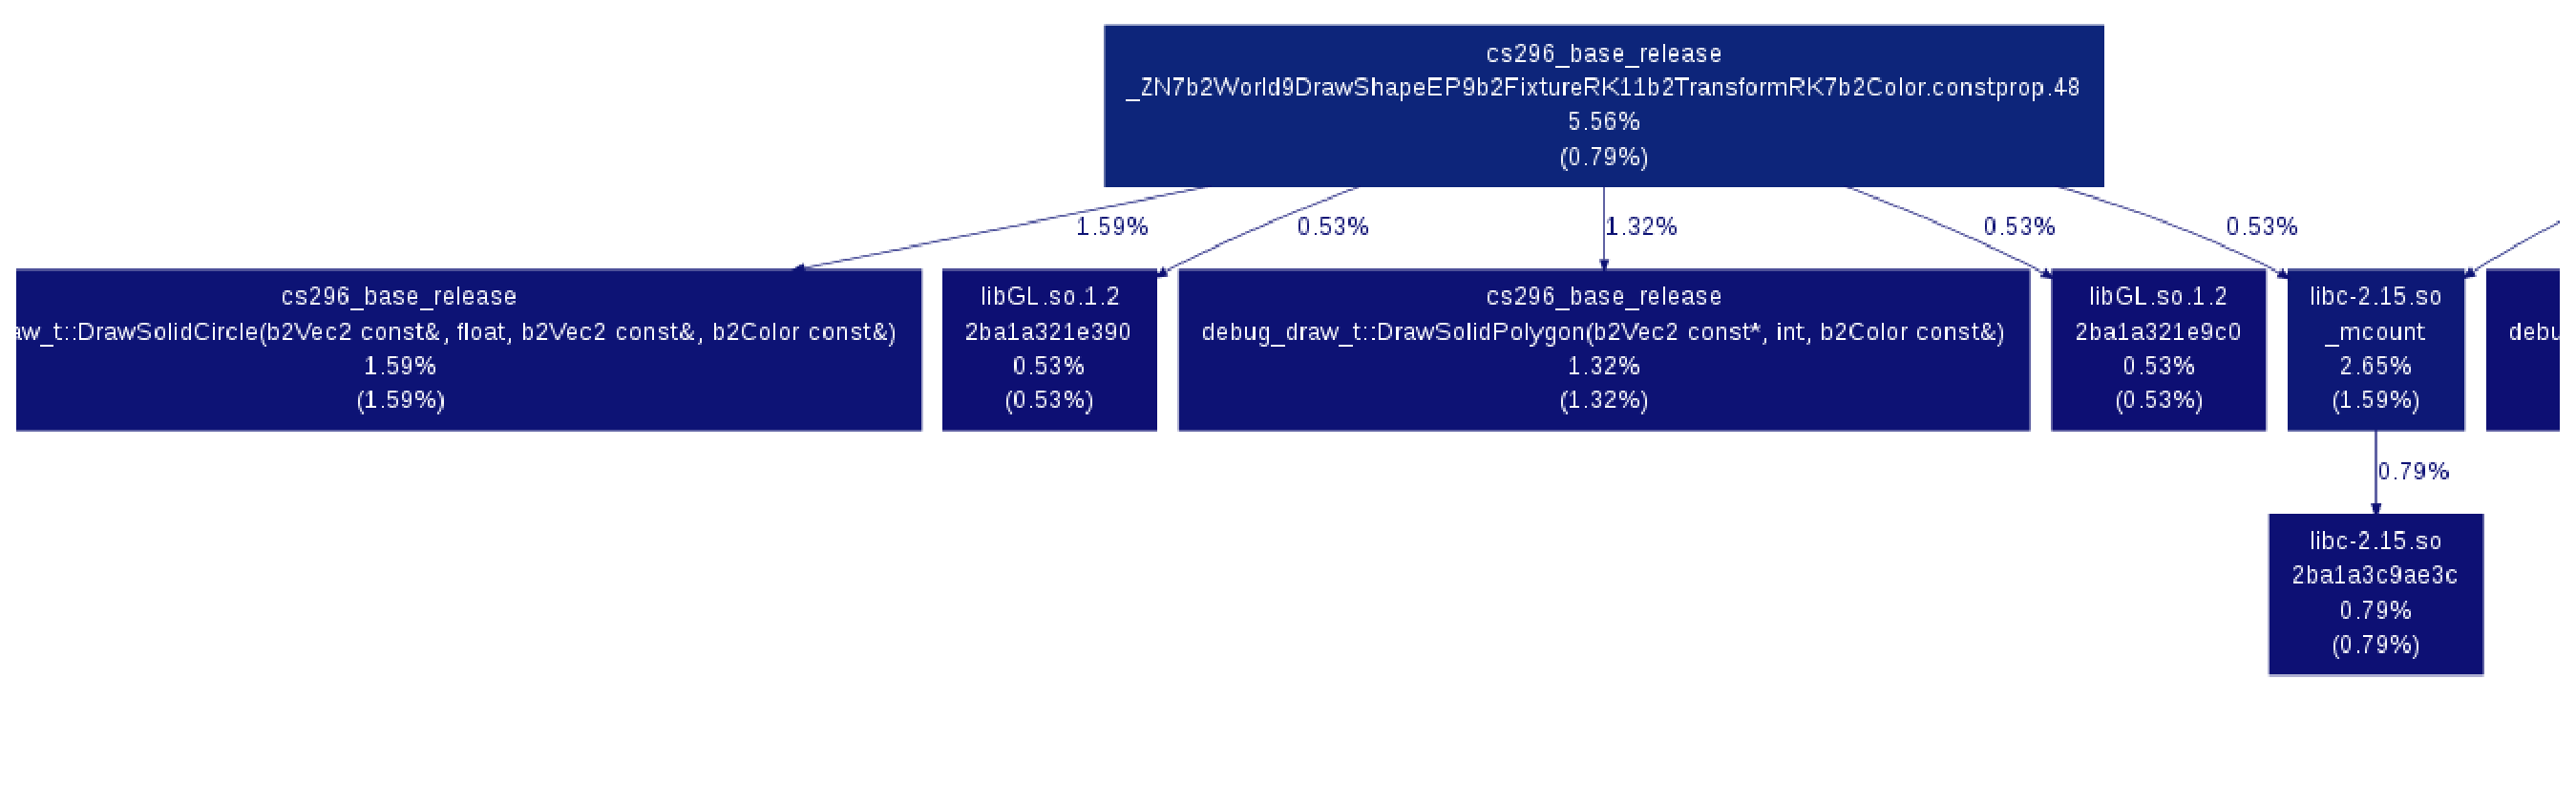
\includegraphics[width=400px]{output_release_0fast}
	\end{center}
	\caption{callgraph for release ofast}
\end{figure}

\begin{figure}
	\begin{center}
		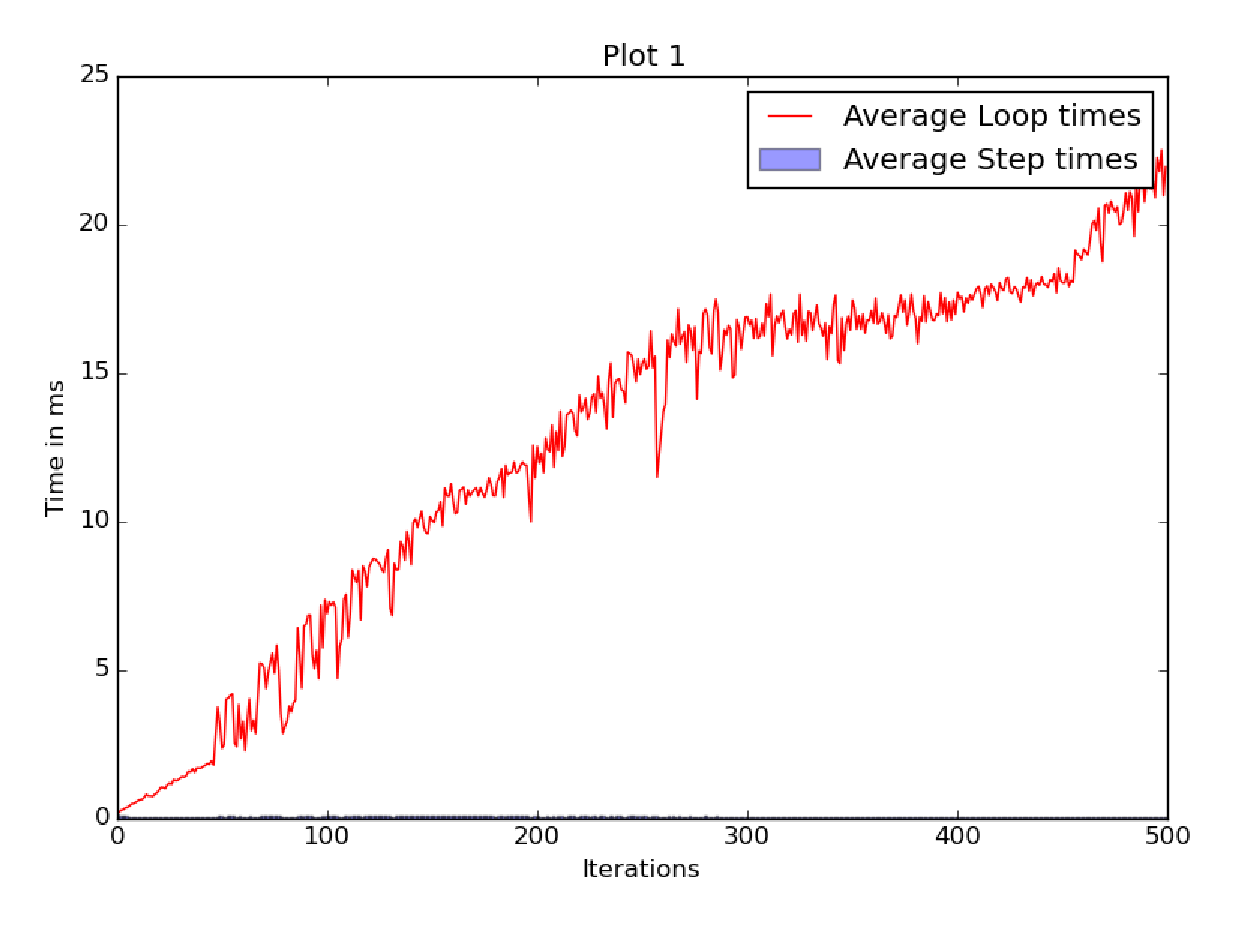
\includegraphics[width=400px]{ofast1}
	\end{center}
	\caption{Figure: Ofast profiling}
\end{figure}

\begin{figure}
	\begin{center}
		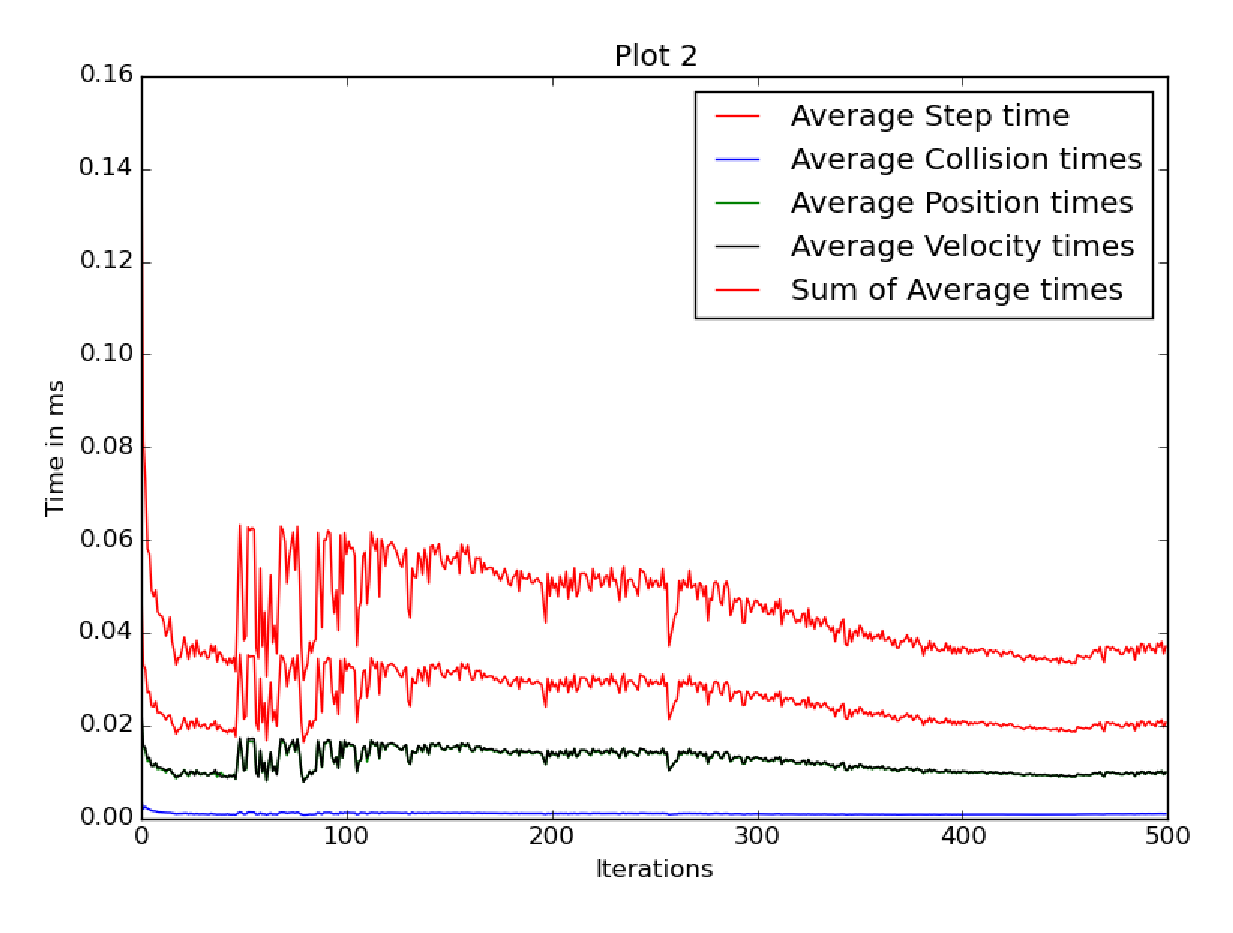
\includegraphics[width=400px]{ofast2}
	\end{center}
	\caption{Figure: Ofast profiling}
\end{figure}

\begin{figure}
	\begin{center}
		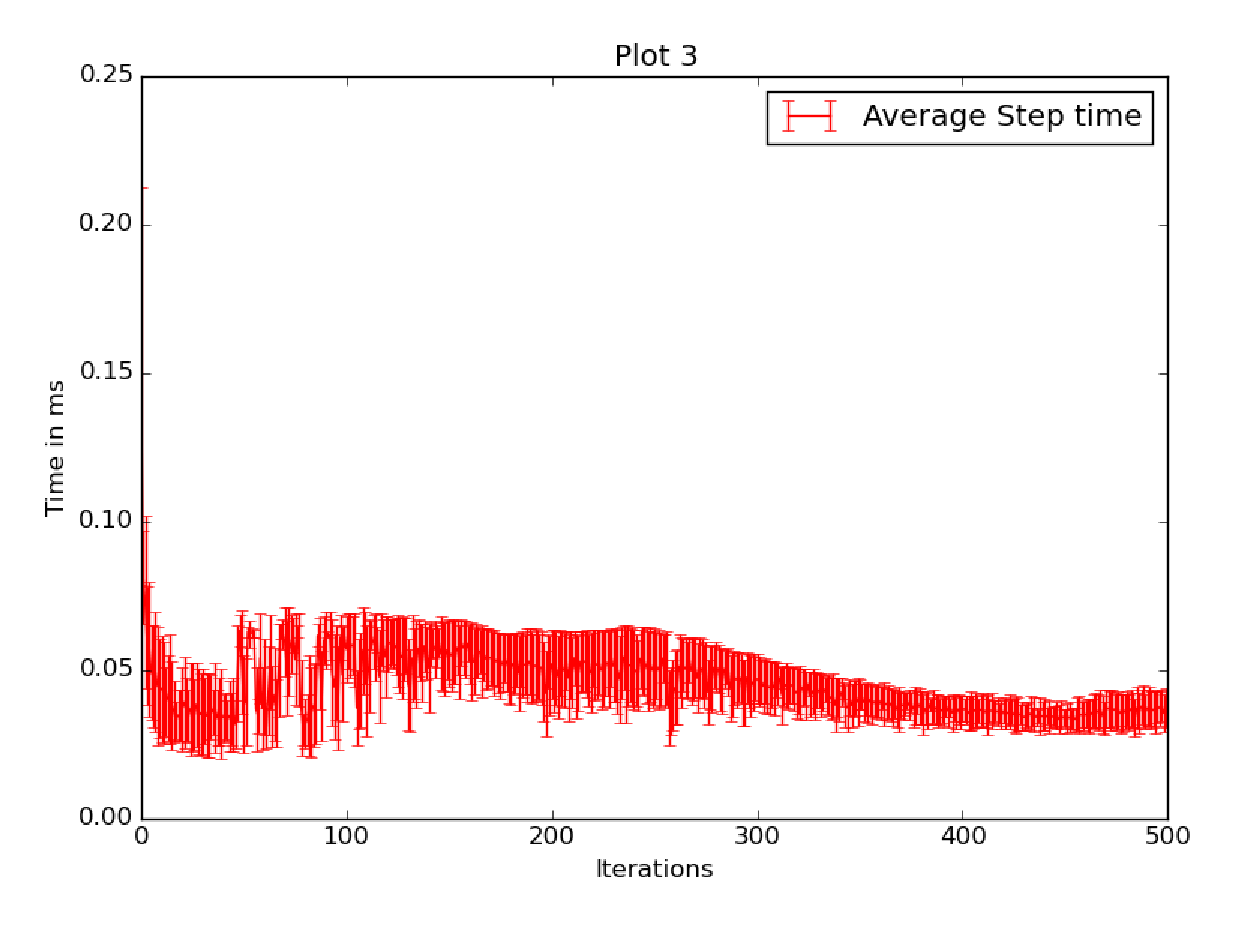
\includegraphics[width=400px]{ofast3}
	\end{center}
	\caption{Figure: Ofast profiling}
\end{figure}

\begin{figure}
	\begin{center}
		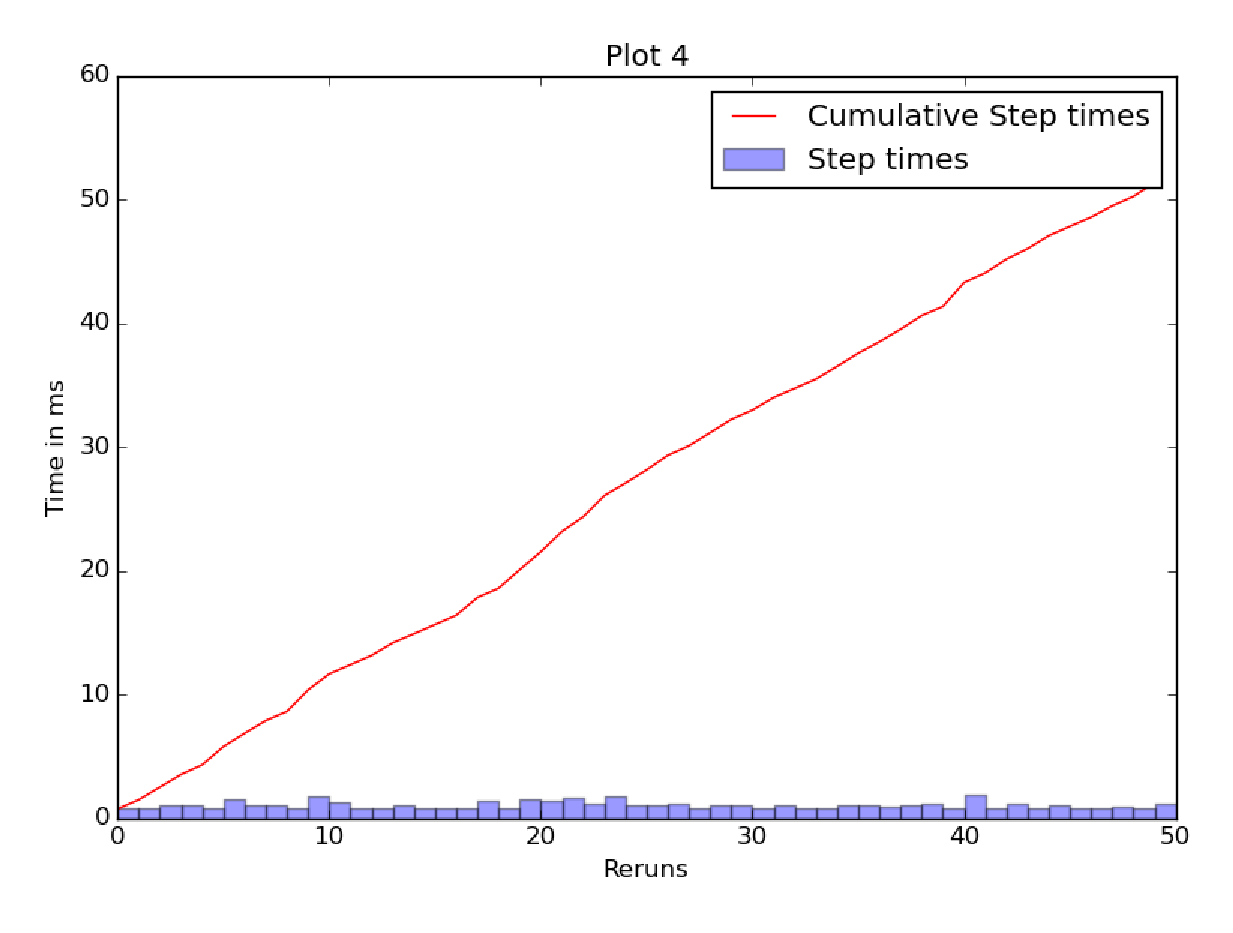
\includegraphics[width=400px]{ofast4}
	\end{center}
	\caption{Figure: Ofast profiling}
\end{figure}

\begin{figure}
	\begin{center}
		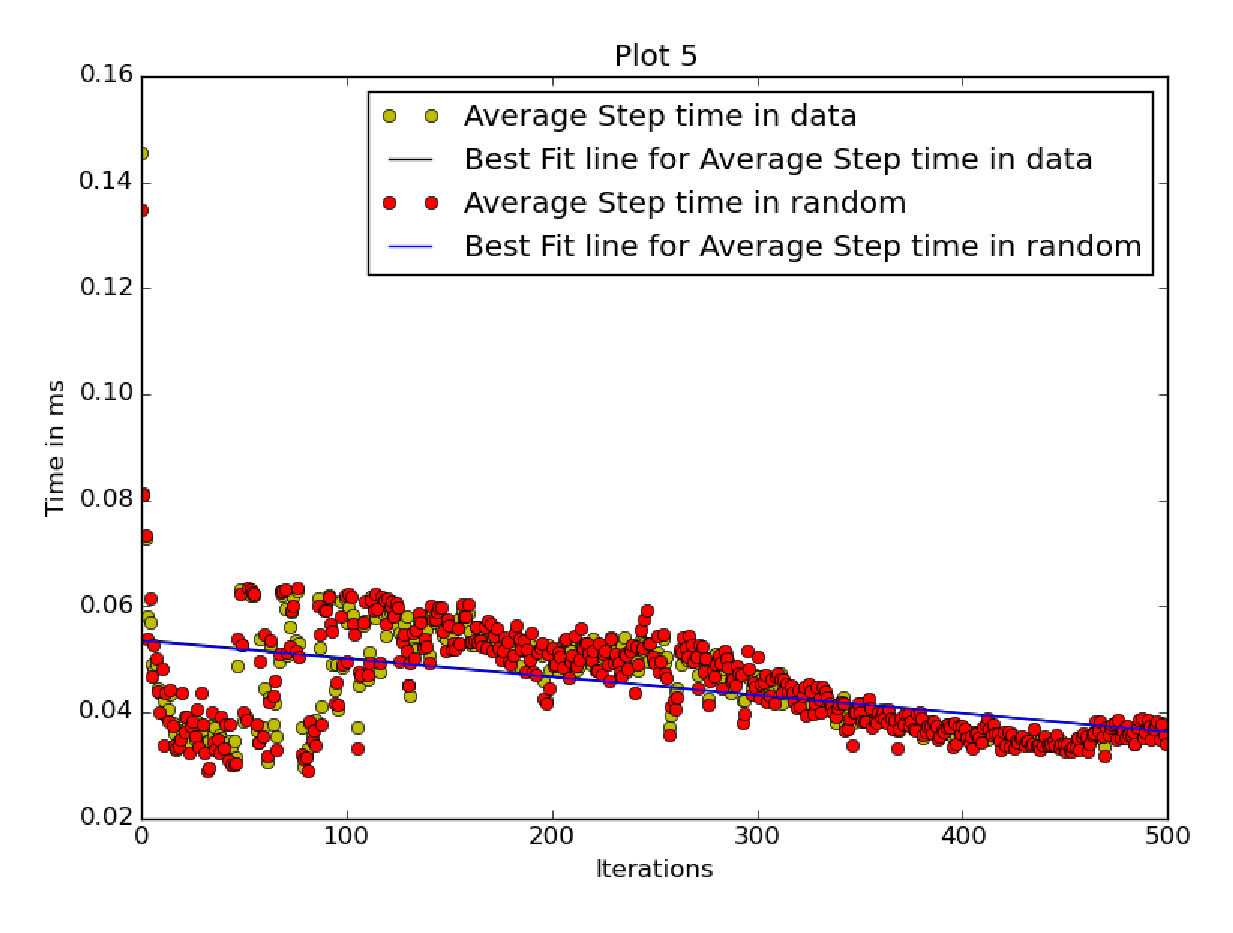
\includegraphics[width=400px]{ofast5}
	\end{center}
	\caption{Figure: Ofast profiling}
\end{figure}

Release Prof Os:\\
Number of Iterations: 10000\\
Average time per step is 0.0353292 ms\\
Average time for collisions is 0.000757077 ms\\
Average time for position updates is 0.0117607 ms\\
Average time for velocity updates is 0.00729658 ms\\
Total loop time is 450.493 ms\\

\begin{figure}
	\begin{center}
		\includegraphics[width=400px]{output_release_0s}
	\end{center}
	\caption{Call graph for release Os}
\end{figure}


Debug Prof:\\
Number of Iterations: 10000\\
Average time per step is 0.174029 ms\\
Average time for collisions is 0.00541188 ms\\
Average time for position updates is 0.0433578 ms\\
Average time for velocity updates is 0.0511959 ms\\
Total loop time is 1874.54 ms\\

\begin{figure}
	\begin{center}
		\includegraphics[width=400px]{output_debug}
	\end{center}
	\caption{Call graph for debug profiling}
\end{figure}

\subsection{Performance Optimization}
After running our code for different optimizations, we found out that -O3 profiling suited best to our code.\\
 Generally Ofast profiling works better than -O3 but for our code -Ofast profiling increased the number of cycles instead of decreasing it.\\ 


\bibliographystyle{plain}
\bibliography{cs296_report_02}
\end{document}
